\chapter{Demo}
This section demonstrates the conversion of a Boolean network from SBML to ERODE and vice versa. Particularly, section 8.1 introduces the network and briefly describes its SBML representation. Section 8.2 gives a short overview of the demo-program.

\section{The example network}
For this demonstration an example network has been created to cover the full extent of the converter's operator interface. The Boolean network is defined as follows:
\begin{itemize}
    \item Given the set of species $S = \{S_1,S_2,S_3\}$
    \item Given the set of update functions $F = \{f_1,f_2,f_3\}$
\end{itemize}
The update functions $F$ are defined as:
\begin{figure}[H]
    \centering
    \[
    \begin{array}{rrrcl}
        f_1(S(t))&=&S_1(t+1) &=& S_2(t) \oplus S_3(t) \\
        f_2(S(t))&=&S_2(t+1) &=& S_1(t) \land \neg{S_3(t)} \\
        f_3(S(t))&=&S_3(t+1) &=& S_1(t) \rightarrow S_2(t)
    \end{array}
    \]
    \caption{The update function definitions}
    \label{fig:exampleBN}
\end{figure}

This network definition was then used to create the \emph{DemoNetwork.sbml}-file. Due to the length of the file, only a few excerpts from it are included in this report. The full length-file can be found in the repository on \href{https://github.com/Unfunctioned/SBML-Converter-for-ERODE}{Github}.

\begin{lstlisting}[language=SBML, caption=The species definitions of the network]
<qual:listOfQualitativeSpecies xmlns:qual=
"http://www.sbml.org/sbml/level3/version1/qual/version1">
  	<qual:qualitativeSpecies qual:compartment="default" 
  	    qual:constant="false"
  	    qual:id="S_1" qual:initialLevel="0"
  	    qual:maxLevel="1"/>
  	<qual:qualitativeSpecies qual:compartment="default" 
  	    qual:constant="false"
  	    qual:id="S_2" qual:initialLevel="0"
  	    qual:maxLevel="1"/>
  	<qual:qualitativeSpecies qual:compartment="default" 
  	    qual:constant="false"
  	    qual:id="S_3" qual:initialLevel="0"
  	    qual:maxLevel="1"/>
</qual:listOfQualitativeSpecies>
\end{lstlisting}

As shown in the SBML-species definitions, all species share the same compartment and are non-constant. Due to being in the Boolean domain $\{0,1\}$, their maximum level has been set to $1$ and they all have been assigned an initial level of $0$.

\begin{lstlisting}[language=SBML, caption=The transition $F_1$ in SBML format]
<qual:transition>
	<qual:listOfInputs>
	    <qual:input qual:id="Input0"
	    qual:qualitativeSpecies="S_2"
	    qual:transitionEffect="none"/>
	    
	    <qual:input qual:id="Input1"
	    qual:qualitativeSpecies="S_3"
	    qual:transitionEffect="none"/>
	</qual:listOfInputs>
	
	<qual:listOfOutputs>
	    <qual:output qual:id="Output0"
	    qual:qualitativeSpecies="S_1"
	    qual:transitionEffect="assignmentLevel"/>
	</qual:listOfOutputs>
	
	<qual:listOfFunctionTerms>
	    <qual:functionTerm qual:resultLevel="1">
	        <math xmlns="http://www.w3.org/1998/Math/MathML">
	            <apply>
	                <xor/>
	                    <apply>
	                        <eq/>
	                        <ci> S_2 </ci>
	                        <cn type="integer"> 1 </cn>
                        </apply>
                        <apply>
                            <eq/>
                            <ci> S_3 </ci>
                            <cn type="integer"> 1 </cn>
                        </apply>
                    </apply>
                </math>
            </qual:functionTerm>
            <qual:defaultTerm qual:resultLevel="0"/>
        </qual:listOfFunctionTerms>
    </qual:transition>
\end{lstlisting}

As seen in the figure above, the list of \emph{outputs} contains a reference to the species $S_1$, since it is updated by the transition. The list of \emph{inputs} contains species $S_2$ and $S_3$, as they are referenced in the update condition, and the function term contains the AST of the update condition. It should be noted, the SBML-representation of the BN used in this example is represented using multi-valued notation, as it is common practice to do so in SBML.

\section{An overview of the demo program}
As it can be seen in figure \ref{fig:demo}, the \emph{SBMLExporter} program, performs can be divided into three segments. In the first segment, the program will use the path to the SBML-file to read the file and parse it to SBML's data representation. The parsed data representation is then available as an \emph{SBMLDocument}-object.

\begin{figure}[H]
    \centering
    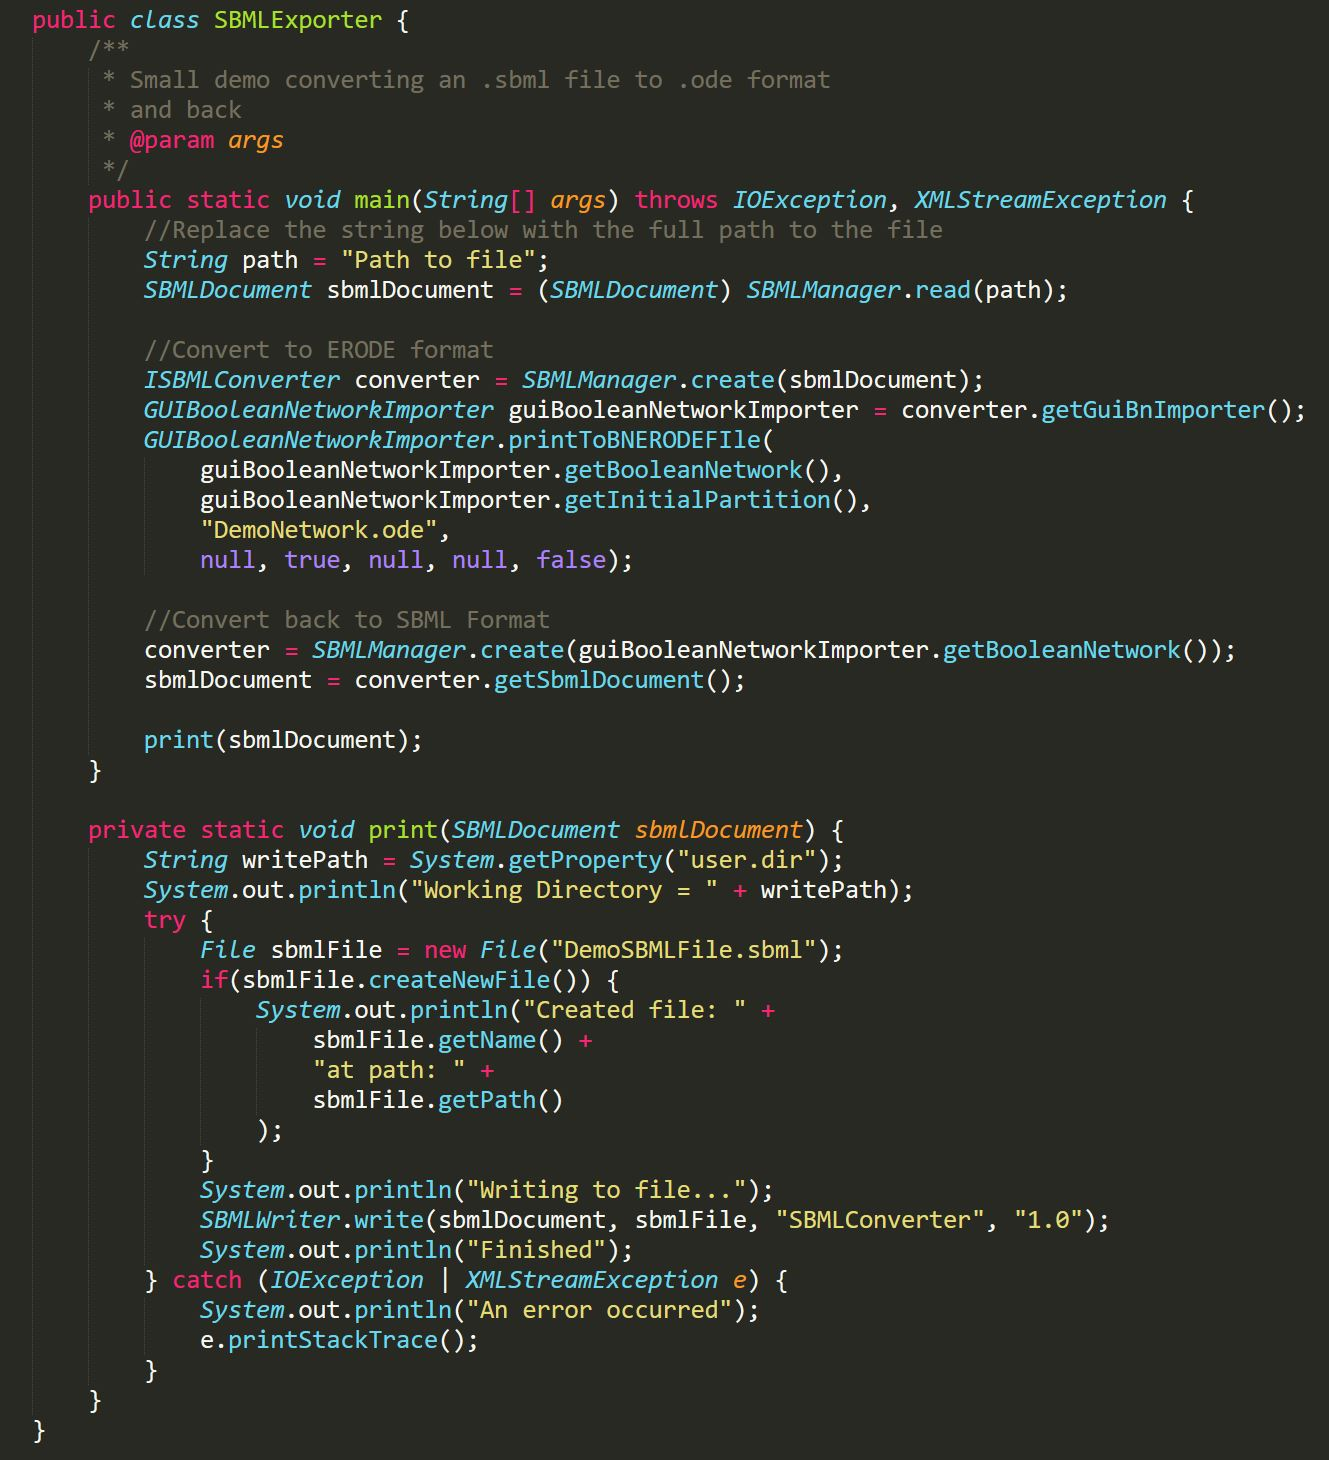
\includegraphics[scale=0.47]{Sections/Images/SBMLExporter.JPG}
    \caption{The demo program}
    \label{fig:demo}
\end{figure}

The second segment uses, the \emph{SBMLDocument} to execute the conversion to ERODE format. The conversion is executed by initialising the \emph{SBMLConverter} using the \emph{SBMLManager}'s \texttt{create()}-method. Once the conversion is complete, the \emph{GUIBooleanNetworkImporter} can be retrieved from the converter. This object contains the network model in ERODE format. ERODE's model representation is then printed to the \emph{DemoNetwork.ode}-file using ERODE's \texttt{printToBNERODEFIle()}-method. This results in the following network in \\
ERODE-format:
\pagebreak
\begin{lstlisting}[language=ERODE, caption=The ERODE formatted network]
begin Boolean network DemoNetwork
 begin init
  S_1
  S_2
  S_3
 end init
begin update functions
  S_1 = (S_2 XOR S_3)
  S_2 = ((S_1 = true)&(S_3 != true))
  S_3 = (S_1 -> (S_2 = true))
end update functions

end Boolean network
\end{lstlisting}

In the last segment of the program shown in figure \ref{fig:demo}, the converts the ERODE representation back to SBML-qual. Just like in the conversion to ERODE format, a new converter is initialized using the \emph{SBMLManager}'s \\
\texttt{create()}-method. This time however, it is given ERODE's data representation instead. Once the conversion is finished, the SBML representation is retrieved by calling the \emph{getSbmlDocument()}-method. The file is then printed to the \emph{DemoSBMLFile}.
When comparing the original input file with the newly generated file, using a file comparison tool, it can be seen that the contents of the file are identical. 